\documentclass[11pt]{beamer}
\usepackage[OT1]{fontenc}
\usepackage[utf8x]{inputenc}
\usepackage[frenchb]{babel}
%\usepackage[dvipsnames]{xcolor}
\usepackage{xcolor}
\usetheme{Cpr}
\title{\textbf{Cahier des charges}}
\subtitle{Communication et conception d'un projet de recherche et/ou développement}
\date{5 Décembre 2012}
\author{Arnaud \textsc{Frèche} \\ Charlotte \textsc{Héricé} \\ Sarai \textsc{Mola}\\ Typhaine  \textsc{Paysan-Lafosse} \\ Joris \textsc{Sansen}}
\institute[Université Bordeaux 1] {Master 2 BioInformatique}
 
\begin{document}

\frame{\titlepage}

\section*{Sommaire}

\begin{frame}
  \tableofcontents
\end{frame}

%%%%%%%%%%%%%%%%%%%%%%%%%%%%%%%%%%
\section{Introduction}			
%%%%%%%%%%%%%%%%%%%%%%%%%%%%%%%%%%

\begin{frame}
	\frametitle{\secname}
	\begin{itemize}
	\item Réseaux Métaboliques.
	\item Mode Élémentaire.
	\end{itemize}
\end{frame}

%%%%%%%%%%%%%%%%%%%%%%%%%%%%%%%%%%
\section{Contexte}			
%%%%%%%%%%%%%%%%%%%%%%%%%%%%%%%%%%

\begin{frame}
	\frametitle{\secname}
	\begin{block}{Sujet}
		\begin{itemize}
		\item Calcul de flux.
		\item \textit{regEfmtool}.
		\end{itemize}
	\end{block}
	\begin{block}{Objectifs}
		\begin{itemize}
		\item Interface Graphique.
		\item Technologies Web : HTML, CSS, JavaScript, PHP.
		\end{itemize}
	\end{block}
\end{frame}

%%%%%%%%%%%%%%%%%%%%%%%%%%%%%%%%%%
\section{État de l'existant}			
%%%%%%%%%%%%%%%%%%%%%%%%%%%%%%%%%%

\begin{frame}
	\frametitle{\secname}
	\begin{block}{Logiciels existants}
		\begin{itemize}
		\item RegEfmtool
		\item CellNetAnalyser
		\item MetaTool
		\end{itemize}
	\end{block}
\end{frame}

%%%%%%%%%%%%%%%%%%%%%%%%%%%%%%%%%%
\section{Besoins	}	
%%%%%%%%%%%%%%%%%%%%%%%%%%%%%%%%%%

\subsection{Besoins fonctionnels}

\begin{frame}
	\frametitle{\subsecname}
	\begin{block}{Besoins fonctionnels}
		\begin{itemize}
		\item Interface Homme-Machine
		\item Chargement des données
		\item Réglage des paramètres et aide utilisateur
		\item Résultats
		\end{itemize}
	\end{block}
\end{frame}

\subsection{Maquette}

\begin{frame}
	\frametitle{\subsecname}
	\begin{figure}[h]
		\begin{center}
		\fbox{
   			\begin{minipage}[c]{0.9\textwidth}
  				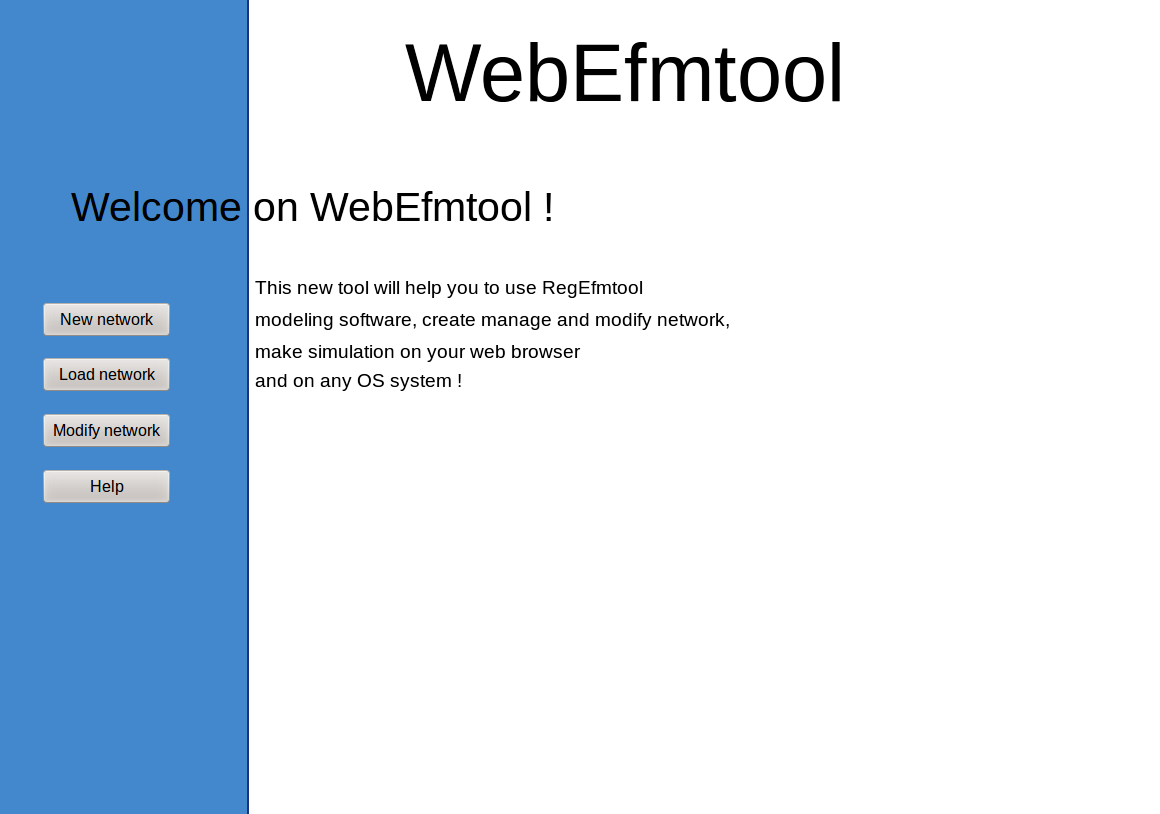
\includegraphics[scale=0.25]{Accueil.png}
			 \end{minipage}}
  		\end{center}	
	 \end{figure}
\end{frame}

\begin{frame}
	\frametitle{\subsecname}
	\begin{figure}[h]
		\begin{center}
		\fbox{
   			\begin{minipage}[c]{0.9\textwidth}
  				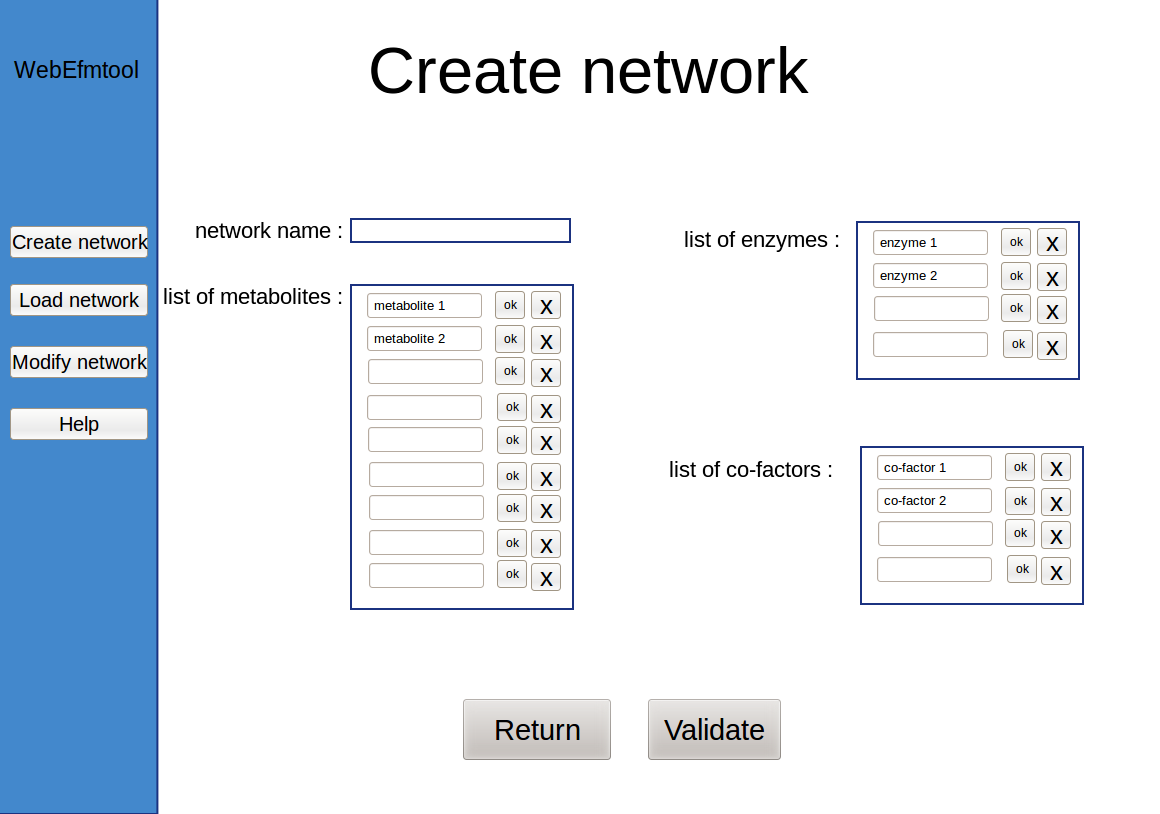
\includegraphics[scale=0.25]{CreateNetwork.png}
			 \end{minipage}}
  		\end{center}	
	 \end{figure}
\end{frame}

\begin{frame}
	\frametitle{\subsecname}
	\begin{figure}[h]
		\begin{center}
		\fbox{
   			\begin{minipage}[c]{0.9\textwidth}
  				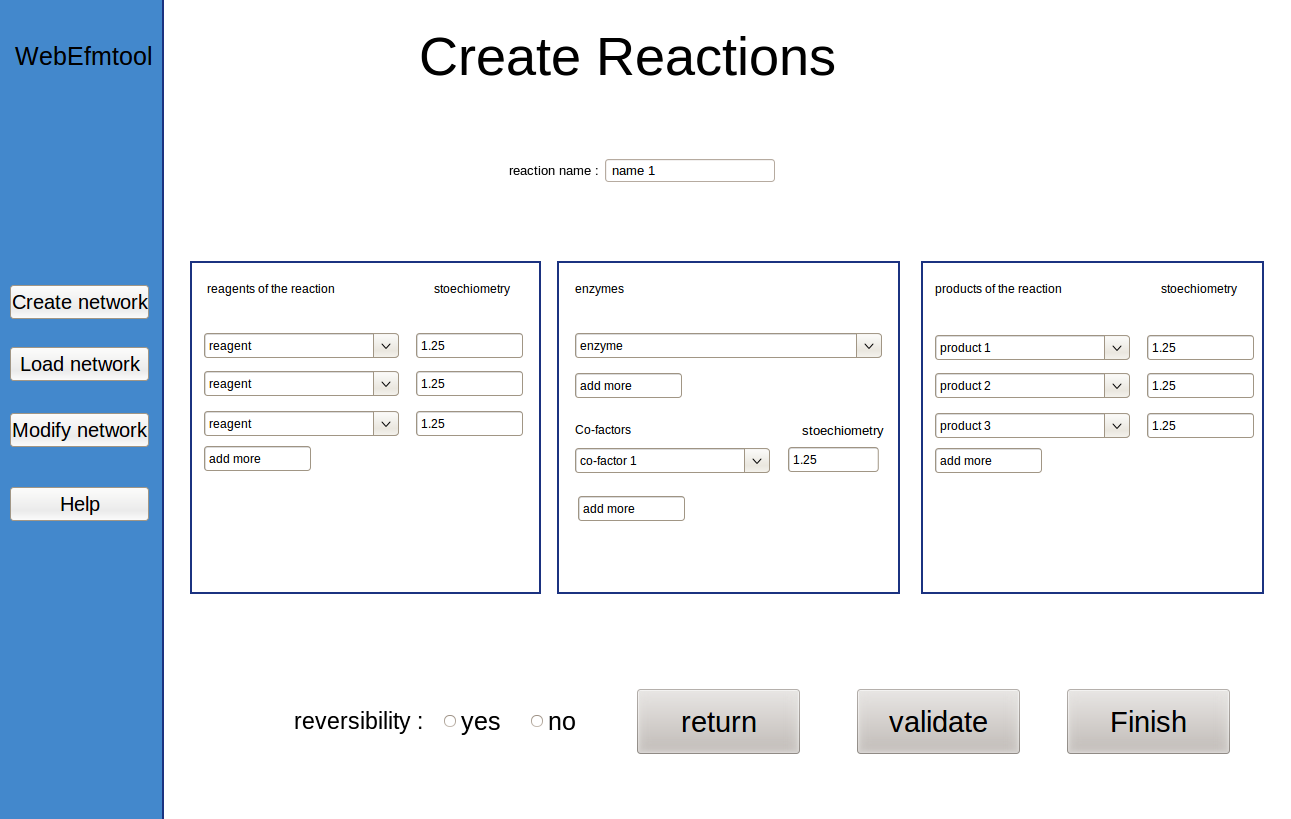
\includegraphics[scale=0.20]{CreateReac.png}
			 \end{minipage}}
  		\end{center}	
	 \end{figure}
\end{frame}

\begin{frame}
	\frametitle{\subsecname}
	\begin{figure}[h]
		\begin{center}
		\fbox{
   			\begin{minipage}[c]{0.9\textwidth}
  				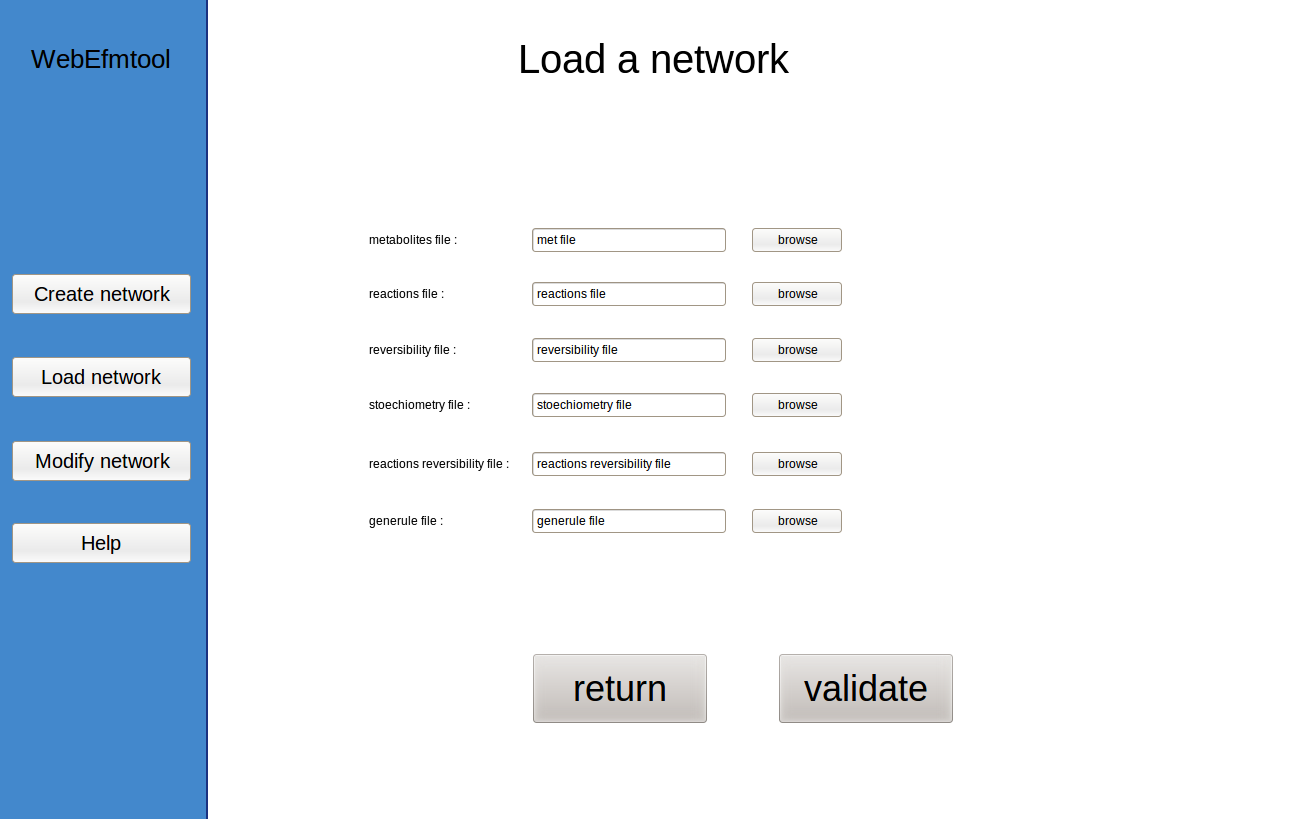
\includegraphics[scale=0.25]{Load.png}
			 \end{minipage}}
  		\end{center}	
	 \end{figure}
\end{frame}

\begin{frame}
	\frametitle{\subsecname}
	\begin{figure}[h]
		\begin{center}
		\fbox{
   			\begin{minipage}[c]{0.9\textwidth}
  				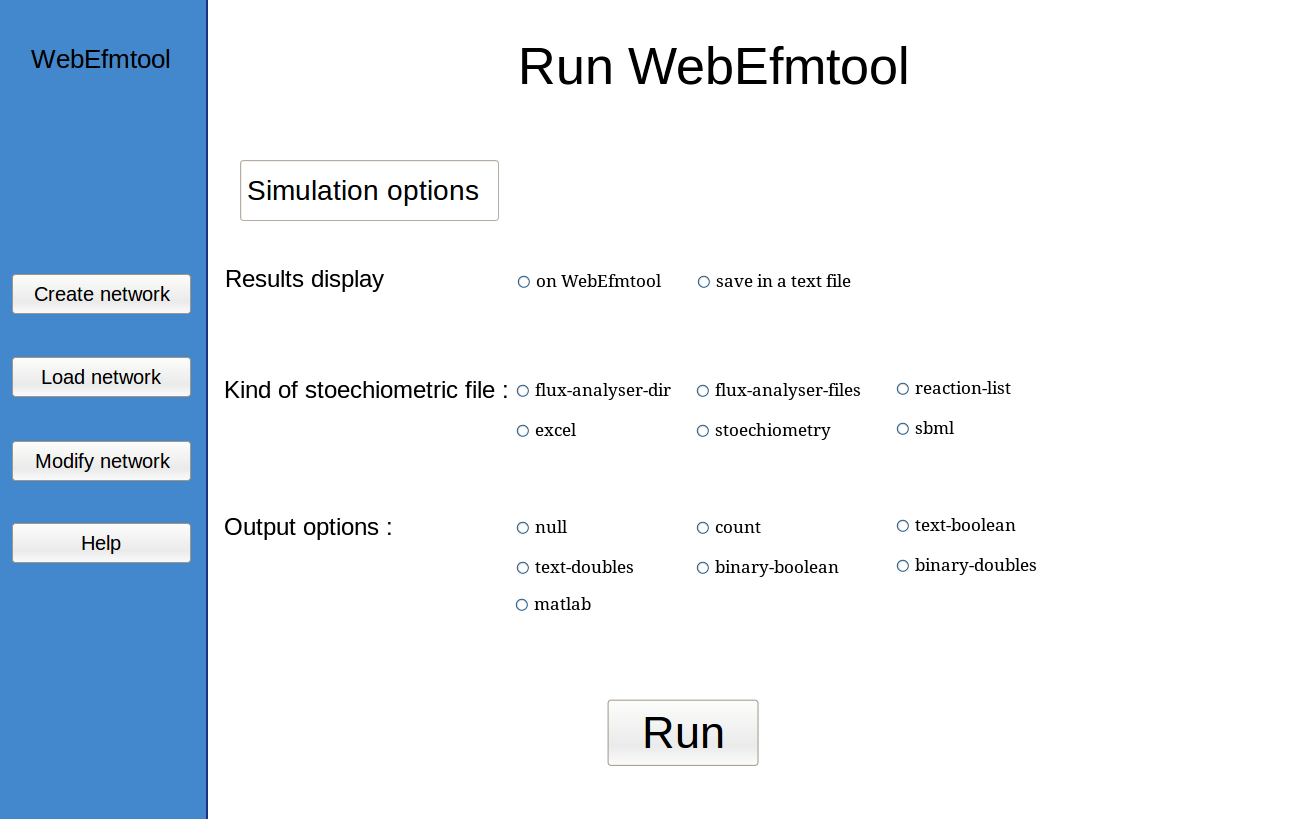
\includegraphics[scale=0.25]{Run.png}
			 \end{minipage}}
  		\end{center}	
	 \end{figure}
\end{frame}

\subsection{Besoins non fonctionnels}

\begin{frame}
	\frametitle{\subsecname}
	\begin{block}{Besoins non fonctionnels}
		\begin{itemize}
		\item Portabilité
		\item Sécurité et robustesse
		\item Temps de calcul
		\item Documentation
		\end{itemize}
	\end{block}
\end{frame}

%%%%%%%%%%%%%%%%%%%%%%%%%%%%%%%%%%
\section{Choix et justifications	}	
%%%%%%%%%%%%%%%%%%%%%%%%%%%%%%%%%%

\begin{frame}
	\frametitle{\secname}
	\begin{block}{}
		\begin{itemize}
		\item Langages
		\item Accessibilité
		%\item Base de données 
		\end{itemize}
	\end{block}
\end{frame}


\end{document}